\chapter{Security Features and Threat Model}
%%%%%%%%%%%%%%%%%%%%%%%%%%%%%%%%%%%%%%%%%
\section{Introduction}
This chapter describes the security features implemented in \projname{} and presents the honest threat model that defines what the system protects and what falls outside its protection boundary. The security model is illustrated in Figure \ref{fig:security_model}.

\begin{figure}[h]
	\centering
	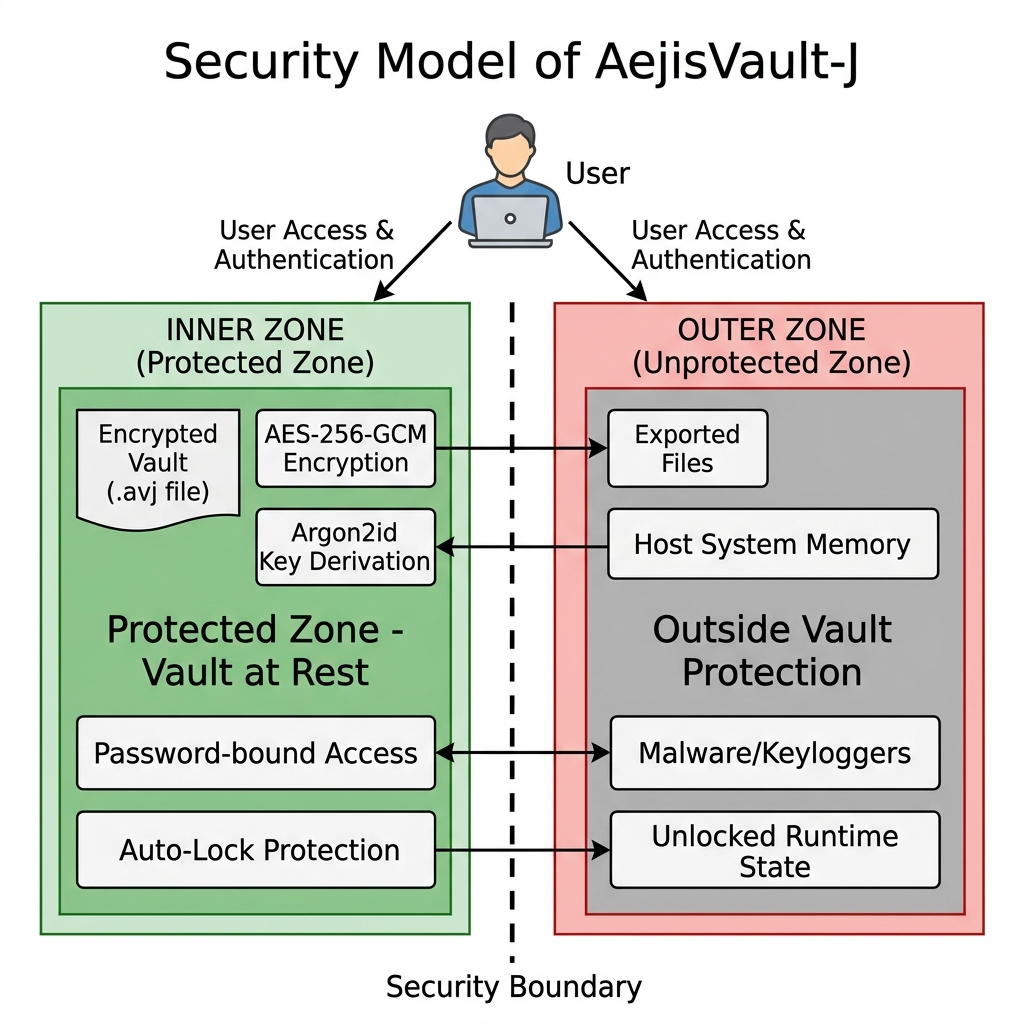
\includegraphics [width=0.85\textwidth] {figures/security_model}
	\caption{Security model of \projname{} showing the boundary between protected vault data and unprotected external data.}
	\label{fig:security_model}	
\end{figure}

%%%%%%%%%%%%%%%%%%%%%%%%%%%%%%%%%%%%%%%%%
\section{Authenticated Encryption}
%%%%%%%%%%%%%%%%%%%%%%%%%%%%%%%%%%%%%%%%%
Authenticated encryption \index{Authenticated encryption} ensures that confidentiality and integrity are both enforced. For a vault system, integrity is as important as secrecy, because corrupted ciphertext should not be silently accepted.

%%%%%%%%%%%%%%%%%%%%%%%%%%%%%%%%%%%%%%%%%
\section{Auto-Lock}
%%%%%%%%%%%%%%%%%%%%%%%%%%%%%%%%%%%%%%%%%
The auto-lock feature \index{Auto-lock} reduces exposure when the user leaves the application idle. This does not eliminate all risk, but it reduces the duration in which sensitive data remains open in memory and in the interface state.

%%%%%%%%%%%%%%%%%%%%%%%%%%%%%%%%%%%%%%%%%
\section{Key Wiping}
%%%%%%%%%%%%%%%%%%%%%%%%%%%%%%%%%%%%%%%%%
The application attempts to clear in-memory copies of sensitive key material after use. This is beneficial but should be understood as best-effort mitigation rather than a guarantee, because runtime environments may retain intermediate copies in internal structures.

%%%%%%%%%%%%%%%%%%%%%%%%%%%%%%%%%%%%%%%%%
\section{Export Warnings}
%%%%%%%%%%%%%%%%%%%%%%%%%%%%%%%%%%%%%%%%%
Since exported files are outside vault protection, the application warns users when they intentionally remove content from secure storage. This helps preserve the clarity of the security model.

%%%%%%%%%%%%%%%%%%%%%%%%%%%%%%%%%%%%%%%%%
\section{Password Strength Checking}
%%%%%%%%%%%%%%%%%%%%%%%%%%%%%%%%%%%%%%%%%
Password strength feedback is included to guide users toward better vault passwords \cite{bonneau_passwords, nist_password}. Strong passwords increase the work factor of brute-force attacks, especially when combined with Argon2id.

%%%%%%%%%%%%%%%%%%%%%%%%%%%%%%%%%%%%%%%%%
\section{Hardware-Backed Key Protection}
%%%%%%%%%%%%%%%%%%%%%%%%%%%%%%%%%%%%%%%%%
The major project introduces hardware-backed key protection \index{Hardware key protection} as an additional layer of defense. When enabled, the Master Vault Key is wrapped using the operating system's native keystore (Windows-ROOT, macOS KeychainStore, or Linux PKCS\#11). This means that even if an attacker obtains the encrypted vault file, they cannot extract the master key without access to the specific machine's keystore. The system supports three modes: software-only (default), OS keystore, and OS keystore with software fallback. Mode changes are recorded in the audit log for accountability.

%%%%%%%%%%%%%%%%%%%%%%%%%%%%%%%%%%%%%%%%%
\section{Access Audit Logging}
%%%%%%%%%%%%%%%%%%%%%%%%%%%%%%%%%%%%%%%%%
The audit logging system \index{Audit logging} records every security-relevant operation: vault creation, opening, closing, file imports, deletions, renames, password changes, and key protection mode changes. Each event is timestamped and stored within the encrypted vault itself, ensuring that the audit trail receives the same cryptographic protection as vault data. The audit log supports search, filtering by event type, and export to CSV for external analysis. This feature is essential for enterprise compliance and for detecting unauthorized access patterns.

%%%%%%%%%%%%%%%%%%%%%%%%%%%%%%%%%%%%%%%%%
\section{Protected Assets}
%%%%%%%%%%%%%%%%%%%%%%%%%%%%%%%%%%%%%%%%%
The system protects the vault while it is stored as an encrypted file and while it is transferred between locations. It also raises the cost of offline brute-force attempts by using Argon2id and AES-GCM correctly.

%%%%%%%%%%%%%%%%%%%%%%%%%%%%%%%%%%%%%%%%%
\section{Out of Scope}
%%%%%%%%%%%%%%%%%%%%%%%%%%%%%%%%%%%%%%%%%
The system does not protect exported files, malware-infected endpoints, keyloggers, memory forensics, or the unlocked runtime state. If a hostile program runs on the host, it may still observe user activity or memory contents.

%%%%%%%%%%%%%%%%%%%%%%%%%%%%%%%%%%%%%%%%%
\section{Boundary of Responsibility}
%%%%%%%%%%%%%%%%%%%%%%%%%%%%%%%%%%%%%%%%%
The boundary of responsibility is a central academic point in the project. Good security software must state clearly what it protects and what it does not protect. \projname{} is designed to be honest in this regard.

\begin{table}[h]
\centering
\caption{Security model summary of \projname{}}
\begingroup
\renewcommand{\arraystretch}{1.3}
\begin{tabular}{l l}
\hline
\rowcolor[HTML]{67FD9A}
{\bfseries Category} & {\bfseries Status} \\
\hline
\rowcolor[HTML]{EFEFEF}
Vault at rest & Protected by AES-256-GCM and password-derived key wrapping \\
\hline
Vault transfer/storage as a file & Protected as an encrypted container \\
\hline
\rowcolor[HTML]{EFEFEF}
Brute-force resistance & Improved by Argon2id and strong password guidance \\
\hline
Exported files & Not protected by the vault \\
\hline
\rowcolor[HTML]{EFEFEF}
Malware/keyloggers & Not protected \\
\hline
Memory forensics & Not guaranteed to be protected \\
\hline
\rowcolor[HTML]{EFEFEF}
Unlocked vault state & Exposed to the current runtime trust boundary \\
\hline
\end{tabular}
\endgroup
\label{tab:security-model}
\end{table}
